\section{Introducción a tipos sesión}

\begin{frame}{Introducción a tipos sesión}

	El desarrollo de software distribuido se enfoca principalmente en la
	integración, cooperación y comunicación de componentes en un sistema.

	\bigskip

	Dificultades:
	\begin{itemize}
		\item{Desafío tecnológico}
		\item{\textbf<2>{Razonamiento sobre el sistema}}
		\pause
	\end{itemize}
\end{frame}

\begin{frame}{Introducción a tipos sesión}
	\begin{figure}
		\centering
		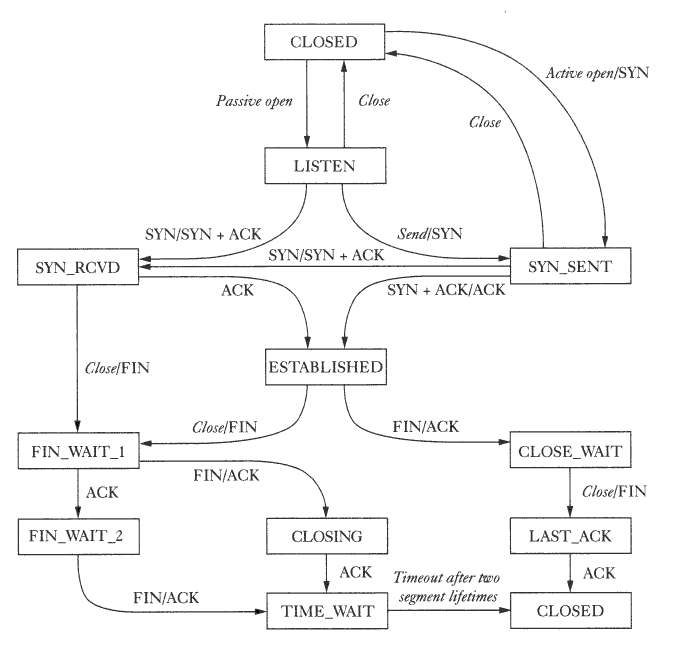
\includegraphics[width=0.6\textwidth]{images/tcp-state-diagram.png}
		\caption{Diagrama de estados para protocolo \textsc{TCP}}
	\end{figure}
\end{frame}

\begin{frame}{Introducción a tipos sesión}

	Esto dio lugar a:

	\begin{itemize}
		\item Desarrollo de técnicas de descripción de interfaces
		\item Soporte a nivel de lenguajes de programación para el desarrollo de aplicaciones correctas por construcción
	\end{itemize}

	\pause

	Los tipos comportamentales, tales como los \textbf{tipos de sesión} constituyen
	un ejemplo paradigmático de esta línea de trabajo.
\end{frame}

\begin{frame}{Introducción a tipos sesión}
	\begin{figure}
		\centering
		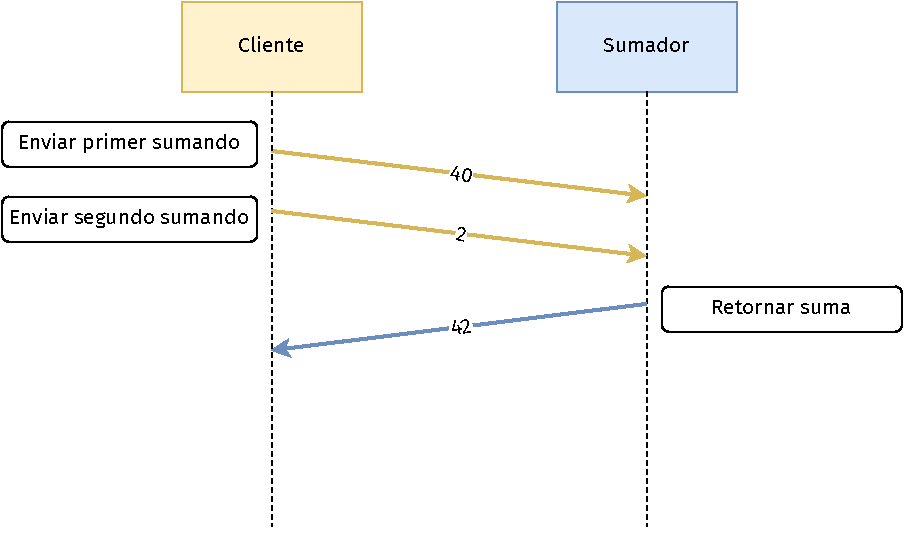
\includegraphics[width=0.9\textwidth]{images/sum-diagram.pdf}
		\caption{Ejemplo de comunicación para un servicio sumador}
	\end{figure}
\end{frame}
